\chapter{त्रिविम रसायन: किरैलता और समावयवी}\label{ch:g12:stereochemistry}

पुदीने की पत्तियों और विलायती जीरे के बीजों की गंध में कोई समानता नहीं: एक च्युइंग गम की
ताज़ा गंध है, दूसरी विलायती जीरे वाली डबलरोटी की गरम गंध। फिर भी हर गंध के लिए ज़िम्मेदार
\omterm{def:g7:atoms-and-molecules:molecule}{अणु} वही कार्वोन है, उन्हीं \omterm{def:g7:atoms-and-molecules:atom}{परमाणुओं} से बना जो उसी क्रम में आबंधित हैं।
दोनों कार्वोन केवल वैसे ही भिन्न हैं जैसे बायाँ हाथ
दाएँ हाथ से भिन्न होता है: हर एक दूसरे का दर्पण-प्रतिबिंब है।
हमारी नाक, जो स्वयं ``हस्तता'' वाले \omterm{def:g7:atoms-and-molecules:molecule}{अणुओं} से बनी है, उन्हें अलग
पहचान लेती है। यह अध्याय \omterm{def:g7:atoms-and-molecules:molecule}{अणुओं} को तीन विमाओं में देखना सिखाता है।

\begin{recall}
\omterm{def:g7:atoms-and-molecules:molecule}{अणुओं} की आकृति, और वे पच्चर और डैश जो उन्हें दिक्स्थान में
दर्शाते हैं (\cref{ch:g10:lewis-and-shape})। \omterm{def:g11:organic-skeletons:isomer}{संरचनात्मक समावयवी}
(\cref{ch:g11:organic-skeletons})। \omterm{def:g11:functional-groups:functional-group}{क्रियात्मक समूह}
(\cref{ch:g11:functional-groups})।
\end{recall}

\begin{omfigure}
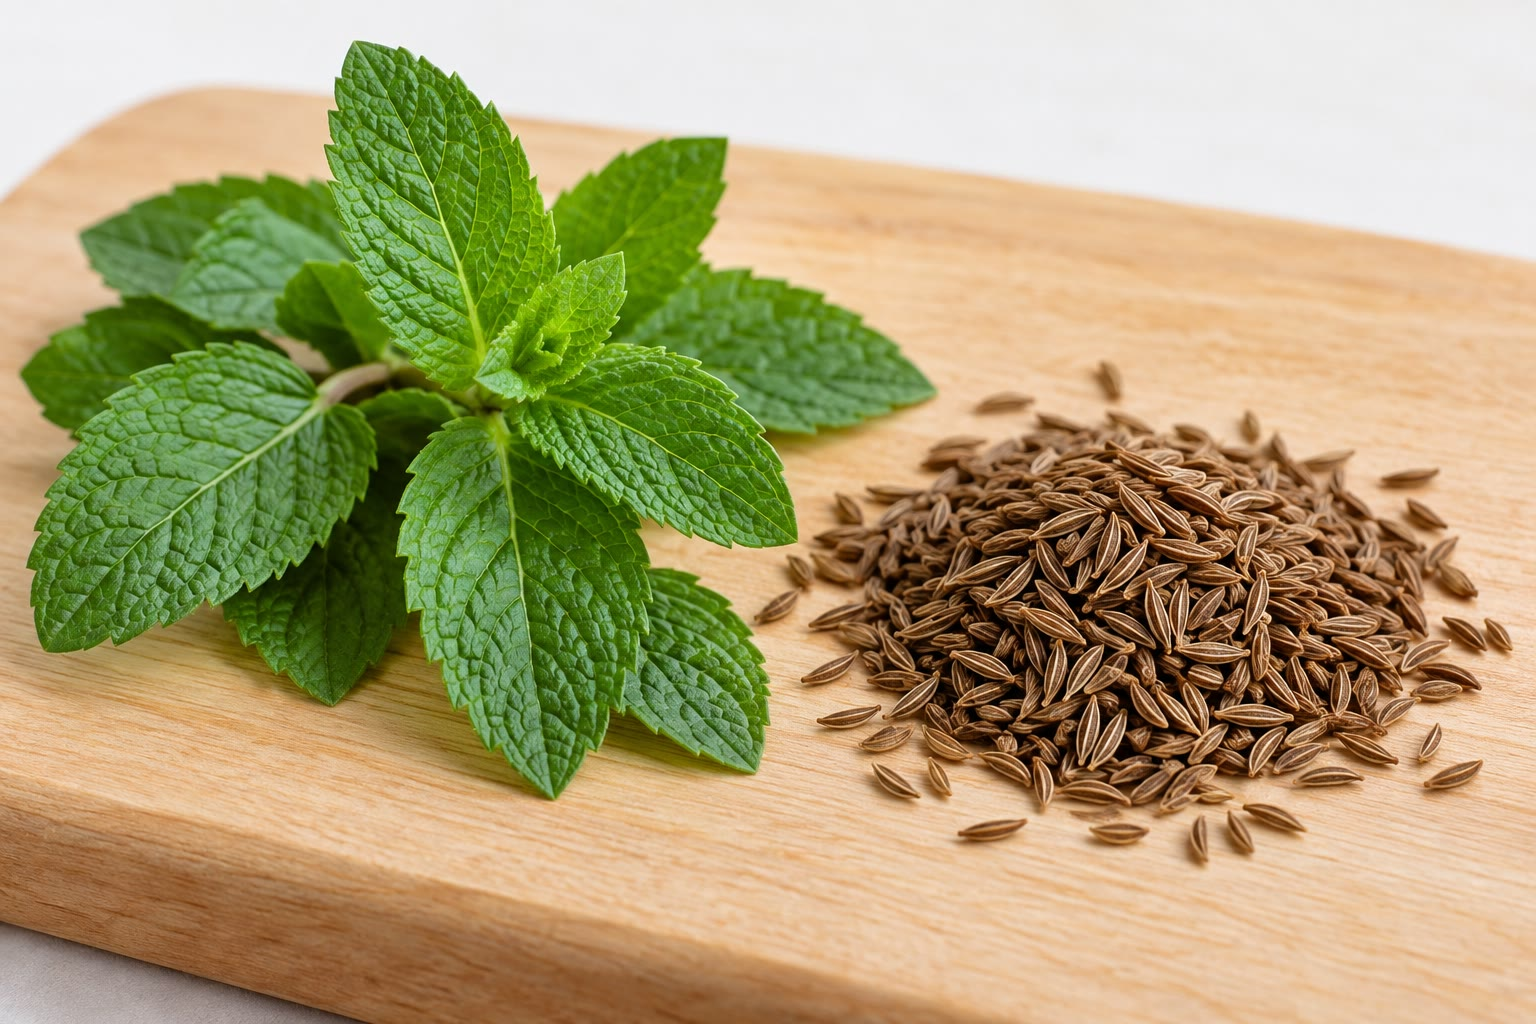
\includegraphics[width=0.48\linewidth]{images/book1/ai/g12-mint-caraway.jpg}

{\small पुदीना और विलायती जीरा: दर्पण-प्रतिबिंब वाले दो \omterm{def:g7:atoms-and-molecules:molecule}{अणु}, दो गंधें।}
\end{omfigure}

\section{दिक्स्थान में अणु}

\begin{definition}[त्रिविम समावयवी]\label{def:g12:stereochemistry:stereoisomer}
\emph{त्रिविम समावयवी}\index{त्रिविम समावयवी} वे \omterm{def:g7:atoms-and-molecules:molecule}{अणु} हैं जिनका
सूत्र और आबंधित \omterm{def:g7:atoms-and-molecules:atom}{परमाणुओं} का क्रम एक ही होता है, और जो केवल
दिक्स्थान में अपने \omterm{def:g7:atoms-and-molecules:atom}{परमाणुओं} की व्यवस्था में भिन्न होते हैं।
\end{definition}

\begin{definition}[क्रैम निरूपण]\label{def:g12:stereochemistry:cram}
चार एकल आबंधों वाले कार्बन \omterm{def:g7:atoms-and-molecules:atom}{परमाणु} के \emph{क्रैम निरूपण}\index{क्रैम निरूपण}
में दो आबंध कागज़ के तल में सादी रेखाओं के रूप में, एक कोण पर,
बनाए जाते हैं; पाठक की ओर इंगित आबंध
ठोस पच्चर के रूप में और दूर इंगित आबंध डैश वाले पच्चर के रूप में।
\end{definition}

\section{किरैलता}

\begin{definition}[किरैल, असममित कार्बन]\label{def:g12:stereochemistry:chiral}
कोई वस्तु या \omterm{def:g7:atoms-and-molecules:molecule}{अणु} \emph{किरैल}\index{किरैल} है यदि उसे
उसके दर्पण-प्रतिबिंब पर अध्यारोपित नहीं किया जा सकता, एक हाथ की तरह। चार भिन्न
\omterm{def:g7:atoms-and-molecules:atom}{परमाणुओं} या समूहों से आबंधित कार्बन \omterm{def:g7:atoms-and-molecules:atom}{परमाणु} एक \emph{असममित
कार्बन}\index{असममित कार्बन} है; उसे अक्सर एक तारे से चिह्नित किया जाता है।
\end{definition}

\begin{proposition}[एक असममित कार्बन अणु को किरैल बना देता है]\label{prop:g12:stereochemistry:one-carbon}
ठीक एक \omterm{def:g12:stereochemistry:chiral}{असममित कार्बन} वाला \omterm{def:g7:atoms-and-molecules:molecule}{अणु} \omterm{def:g12:stereochemistry:chiral}{किरैल} होता है।
\end{proposition}

\begin{proof}
स्वीकृत: \omterm{def:g12:stereochemistry:chiral}{असममित कार्बन} के चारों ओर के चार भिन्न समूहों में से दो को आपस में बदलने पर
दर्पण-प्रतिबिंब मिलता है, और पूरे \omterm{def:g7:atoms-and-molecules:molecule}{अणु} का कोई भी घूर्णन उसे वापस
नहीं ला सकता, क्योंकि चारों समूह भिन्न हैं।
\end{proof}

\begin{definition}[प्रतिबिंबरूपी, रेसेमिक मिश्रण]\label{def:g12:stereochemistry:enantiomer}
वे दो \omterm{def:g12:stereochemistry:stereoisomer}{त्रिविम समावयवी} जो एक-दूसरे के दर्पण-प्रतिबिंब हों और
अध्यारोपित न हो सकें, \emph{प्रतिबिंबरूपी}\index{प्रतिबिंबरूपी} हैं। दो प्रतिबिंबरूपियों
की समान मात्राओं का \omterm{def:g6:pure-substances-and-mixtures:mixture}{मिश्रण} एक \emph{रेसेमिक
मिश्रण}\index{रेसेमिक मिश्रण} है।
\end{definition}

\begin{omfigure}
\setchemfig{atom sep=2.2em}
\begin{tikzpicture}[font=\small]
  \node at (-2.4,0) {\chemfig{C(-[2]COOH)(-[4]H_3C)(<[:-30]OH)(<:[:-150]H)}};
  \node at (2.4,0) {\chemfig{C(-[2]COOH)(-[0]CH_3)(<[:-150]HO)(<:[:-30]H)}};
  \draw[dashed, omDef, thick] (0,-1.5) -- (0,1.6) node[above] {दर्पण};
  \node[anchor=north] at (-2.4,-1.4) {लैक्टिक अम्ल, A};
  \node[anchor=north] at (2.4,-1.4) {उसका दर्पण-प्रतिबिंब, B};
\end{tikzpicture}

{\small \omterm{def:g12:stereochemistry:cram}{क्रैम निरूपण} में लैक्टिक अम्ल, \ce{CH3-CH(OH)-COOH}, के दोनों
\omterm{def:g12:stereochemistry:enantiomer}{प्रतिबिंबरूपी}। केंद्रीय कार्बन असममित है (\ce{H}, \ce{OH},
\ce{CH3}, \ce{COOH})। कोई घूर्णन A को B में नहीं बदलता: वे उतने ही भिन्न हैं
जितना बायाँ और दायाँ हाथ।}
\end{omfigure}

\begin{method}[क्या कोई अणु किरैल है?]\label{met:g12:stereochemistry:chiral}
\begin{enumerate}
  \item \omterm{def:g12:stereochemistry:chiral}{असममित कार्बन} खोजिए: चार भिन्न समूहों वाला
        कार्बन। एक भी नहीं: \omterm{def:g7:atoms-and-molecules:molecule}{अणु} (इस पुस्तक में) \omterm{def:g12:stereochemistry:chiral}{किरैल} नहीं है।
  \item ठीक एक: \omterm{def:g7:atoms-and-molecules:molecule}{अणु} \omterm{def:g12:stereochemistry:chiral}{किरैल} है।
  \item दो या अधिक: \omterm{def:g7:atoms-and-molecules:molecule}{अणु} की किसी एक आकृति में ऐसा तल खोजिए जो उसे दो
        दर्पण-अर्धों में काटे; यदि ऐसा तल है, तो
        \omterm{def:g7:atoms-and-molecules:molecule}{अणु} \omterm{def:g12:stereochemistry:chiral}{किरैल} नहीं है, अन्यथा है।
\end{enumerate}
\end{method}

\begin{remark}[समान गुण, भिन्न गंधें]\label{rem:g12:stereochemistry:same}
% ledger: smell:carvone-R, smell:carvone-S
दो \omterm{def:g12:stereochemistry:enantiomer}{प्रतिबिंबरूपियों} के गलनांक और क्वथनांक, \omterm{def:g6:solutions-and-solubility:solubility}{विलेयता} और स्पेक्ट्रम
एक जैसे होते हैं: किसी ऐसी चीज़ से किया गया हर माप जो
स्वयं \omterm{def:g12:stereochemistry:chiral}{किरैल} नहीं है, दोनों के लिए एक ही परिणाम देता है। वे केवल
तब भिन्न होते हैं जब उनका सामना किसी \omterm{def:g12:stereochemistry:chiral}{किरैल} चीज़ से हो, जैसे ध्रुवित प्रकाश, जिसे वे
विपरीत दिशाओं में घुमाते हैं, या नाक के ग्राही: एक कार्वोन से
पुदीने की गंध आती है, उसके \omterm{def:g12:stereochemistry:enantiomer}{प्रतिबिंबरूपी} से विलायती जीरे की।
\end{remark}

\section{अप्रतिबिंबरूपी}

\begin{definition}[अप्रतिबिंबरूपी]\label{def:g12:stereochemistry:diastereomer}
वे \omterm{def:g12:stereochemistry:stereoisomer}{त्रिविम समावयवी} जो एक-दूसरे के दर्पण-प्रतिबिंब नहीं हैं,
\emph{अप्रतिबिंबरूपी}\index{अप्रतिबिंबरूपी} हैं। \omterm{def:g12:stereochemistry:enantiomer}{प्रतिबिंबरूपियों} के विपरीत,
अप्रतिबिंबरूपियों के भौतिक गुण भिन्न होते हैं।
\end{definition}

\begin{proposition}[त्रिविम समावयवियों की गिनती]\label{prop:g12:stereochemistry:count}
$n$ \omterm{def:g12:stereochemistry:chiral}{असममित कार्बनों} वाले \omterm{def:g7:atoms-and-molecules:molecule}{अणु} के अधिक से अधिक $2^n$ \omterm{def:g12:stereochemistry:stereoisomer}{त्रिविम समावयवी} होते हैं।
जब \omterm{def:g7:atoms-and-molecules:molecule}{अणु} के दो एक जैसे अर्ध हों, तो ये कम होते हैं: तब संयोजनों में से एक में
दर्पण-तल होता है और वह \omterm{def:g12:stereochemistry:chiral}{किरैल} नहीं होता (एक \emph{मेसो} रूप)।
\end{proposition}

\begin{proof}
हर \omterm{def:g12:stereochemistry:chiral}{असममित कार्बन} दूसरों से स्वतंत्र रूप से दो व्यवस्थाएँ ले सकता है:
$2 \times 2 \times \dots \times 2 = 2^n$ संयोजन। जब दो
संयोजन एक ही \omterm{def:g7:atoms-and-molecules:molecule}{अणु} हों, तो गिनती घट जाती है।
\end{proof}

\begin{omfigure}
\setchemfig{atom sep=1.9em}
\begin{tabular}{ccc}
\chemfig{HOOC-[:-30]C(<[:-90]OH)-[:30]C(<[:90]OH)-[:-30]COOH} &
\chemfig{HOOC-[:-30]C(<:[:-90]OH)-[:30]C(<:[:90]OH)-[:-30]COOH} &
\chemfig{HOOC-[:-30]C(<[:-90]OH)-[:30]C(<:[:90]OH)-[:-30]COOH} \\[4pt]
\small L-टार्टरिक अम्ल & \small D-टार्टरिक अम्ल & \small मेसो-टार्टरिक अम्ल \\
\small (\omterm{def:g12:stereochemistry:chiral}{किरैल}) & \small (\omterm{def:g12:stereochemistry:chiral}{किरैल}, L का दर्पण-प्रतिबिंब) & \small (\omterm{def:g12:stereochemistry:chiral}{किरैल} नहीं)
\end{tabular}

{\small टार्टरिक अम्ल के तीन \omterm{def:g12:stereochemistry:stereoisomer}{त्रिविम समावयवी}। L और D
\omterm{def:g12:stereochemistry:enantiomer}{प्रतिबिंबरूपी} हैं; हर एक मेसो रूप का \omterm{def:g12:stereochemistry:diastereomer}{अप्रतिबिंबरूपी} है, जिसकी किसी एक आकृति में
दर्पण-तल होता है: तीन \omterm{def:g12:stereochemistry:stereoisomer}{त्रिविम समावयवी}, $2^2 = 4$ नहीं।}
\end{omfigure}

\begin{history}[पाश्चर हाथ से क्रिस्टल छाँटते हैं, 1848]
1848 में युवा रसायनज्ञ लुई पाश्चर ने आवर्धक लेंस से ``रेसेमिक अम्ल'' के
एक लवण के क्रिस्टल देखे, जो टार्टरिक अम्ल का एक ऐसा रूप था जो
ध्रुवित प्रकाश को किसी भी ओर नहीं घुमाता था। उन्होंने देखा कि क्रिस्टल
दो आकृतियों में थे, जो एक-दूसरे के दर्पण-प्रतिबिंब थीं, और उन्होंने चिमटी से उन्हें
एक-एक करके छाँटा। घोलने पर एक ढेर ने ध्रुवित प्रकाश को दाईं ओर घुमाया,
दूसरे ने उतना ही बाईं ओर: रेसेमिक अम्ल दो दर्पण-प्रतिबिंब \omterm{def:g7:atoms-and-molecules:molecule}{अणुओं} का
\omterm{def:g6:pure-substances-and-mixtures:mixture}{मिश्रण} था। उन्होंने निष्कर्ष निकाला कि \omterm{def:g7:atoms-and-molecules:molecule}{अणुओं} में हस्तता हो सकती है।
\end{history}

\begin{omfigure}
\begin{minipage}[t]{0.36\linewidth}\centering
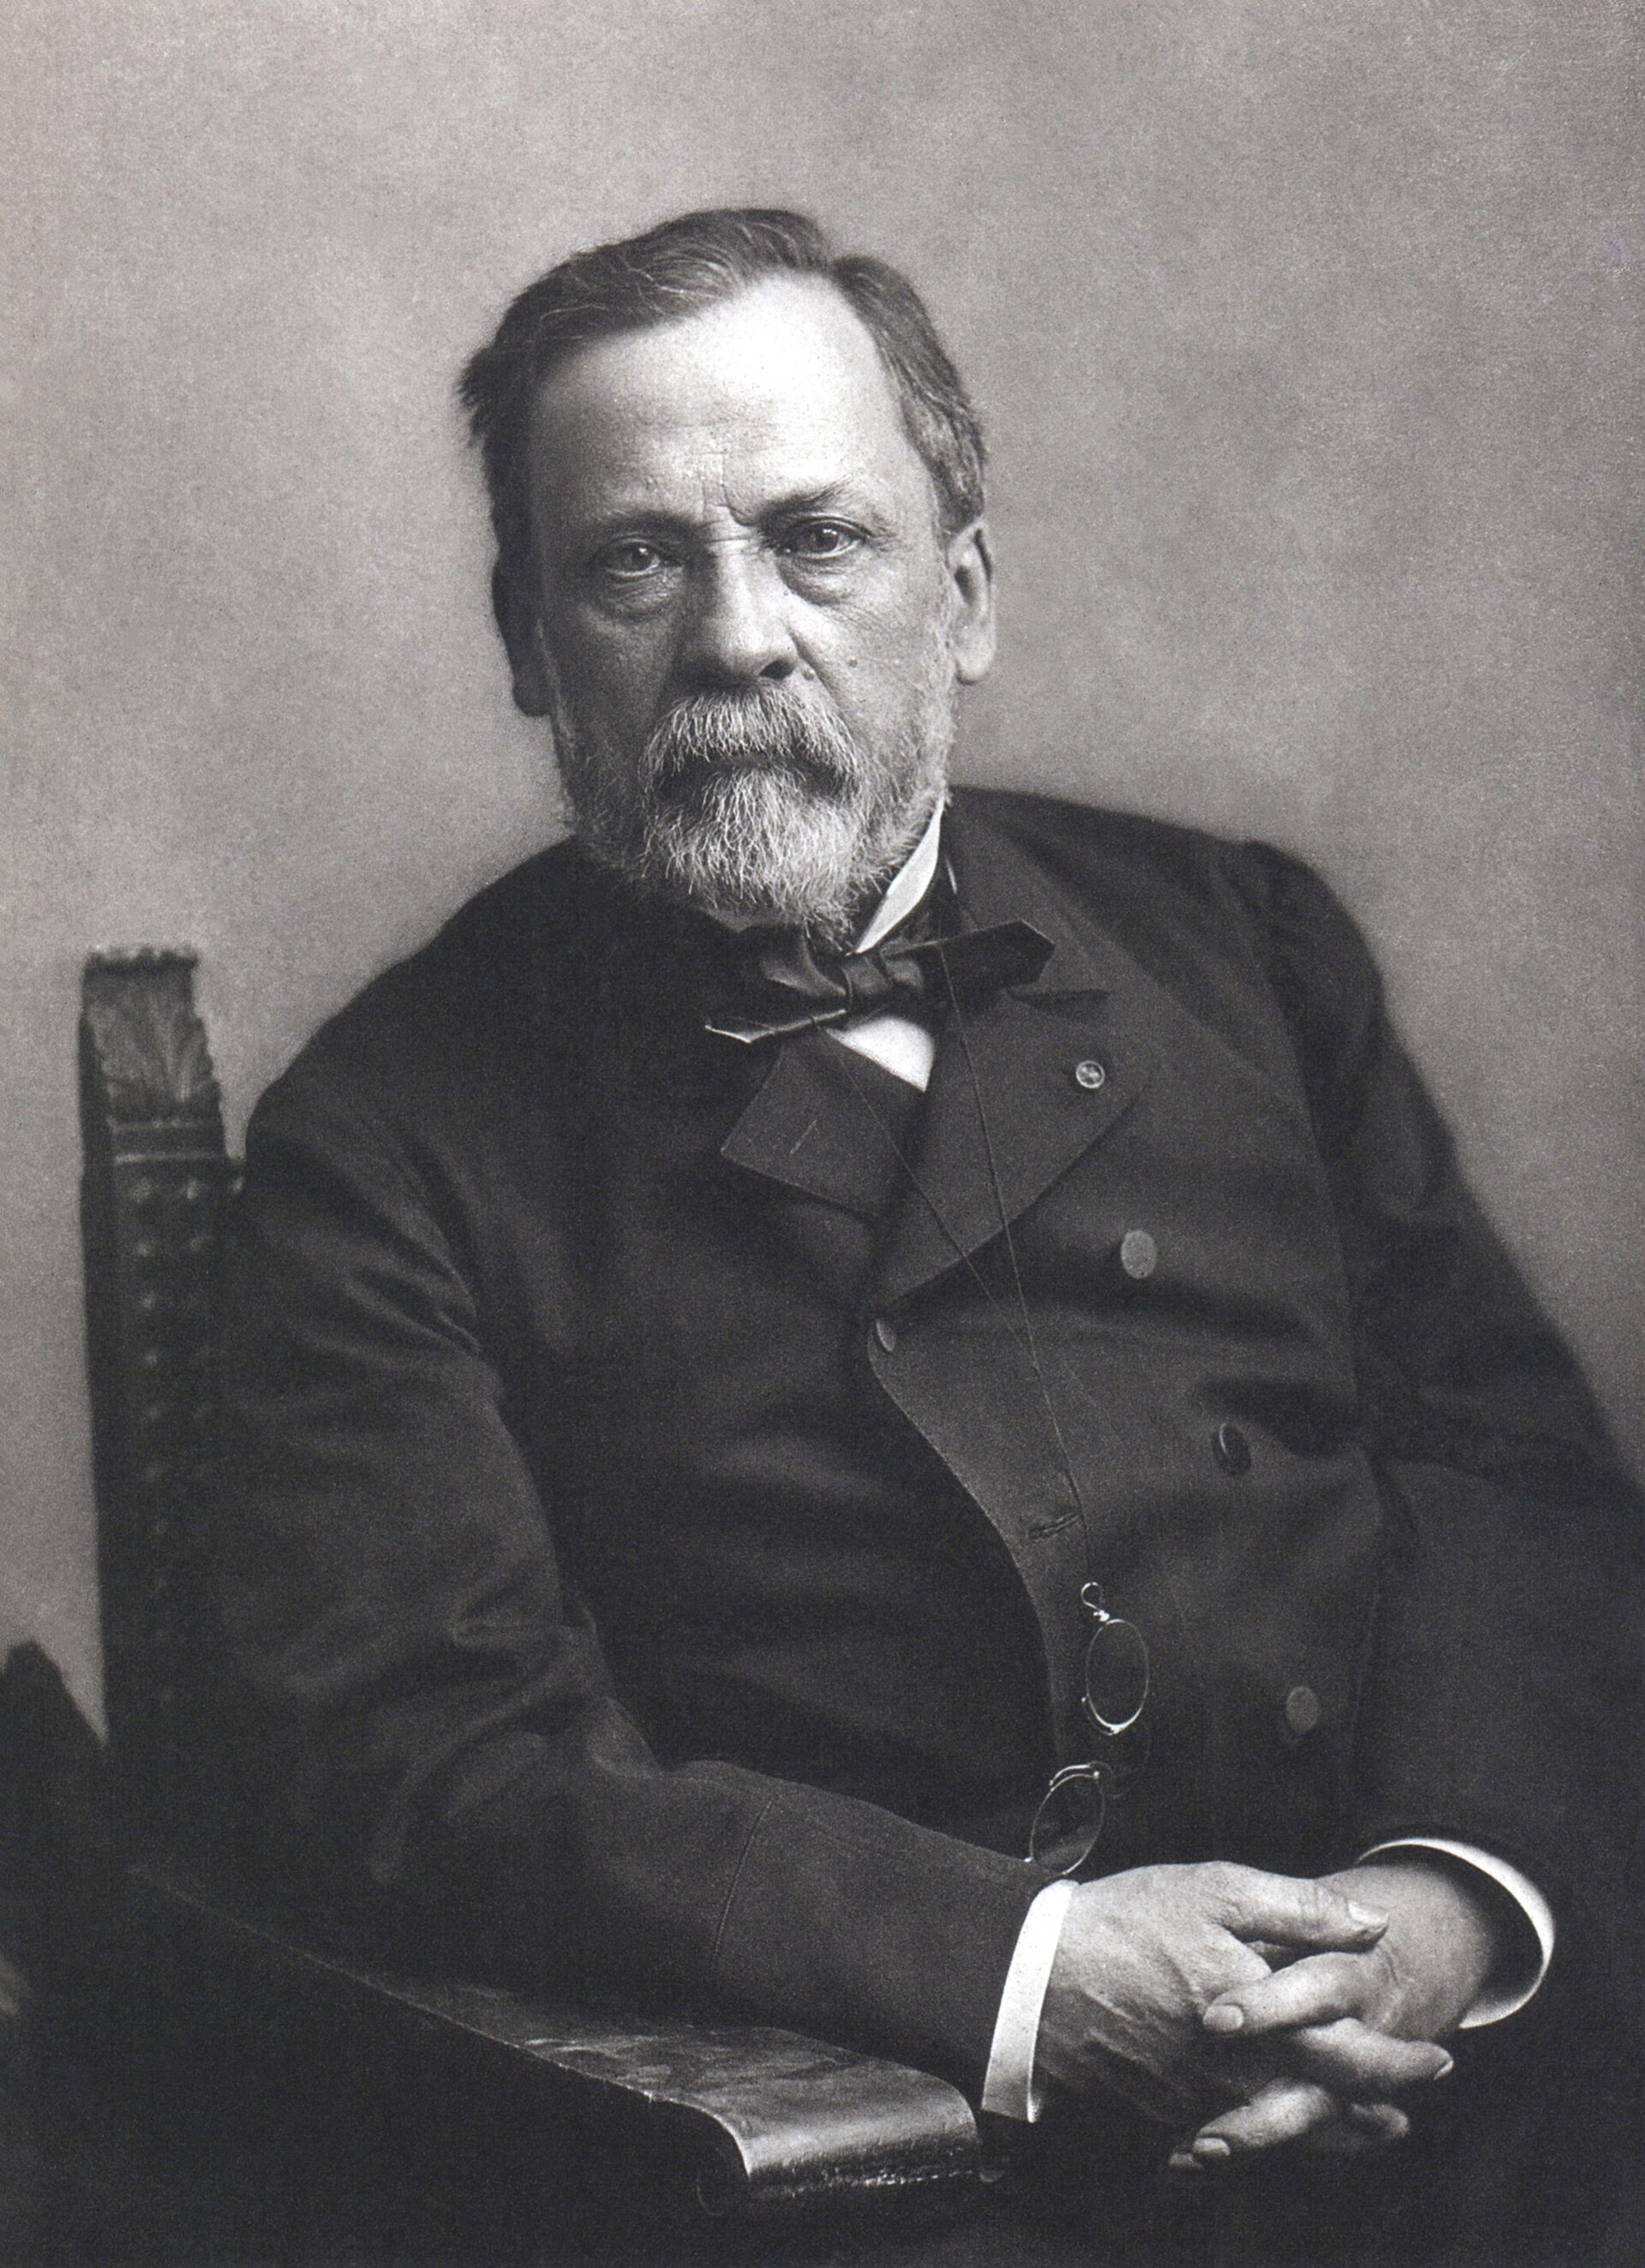
\includegraphics[height=5cm]{images/book1/pasteur.jpg}

{\small लुई पाश्चर (1822--1895), पॉल नादार द्वारा खींचा गया फ़ोटो।}
\end{minipage}\qquad
\begin{minipage}[t]{0.36\linewidth}\centering
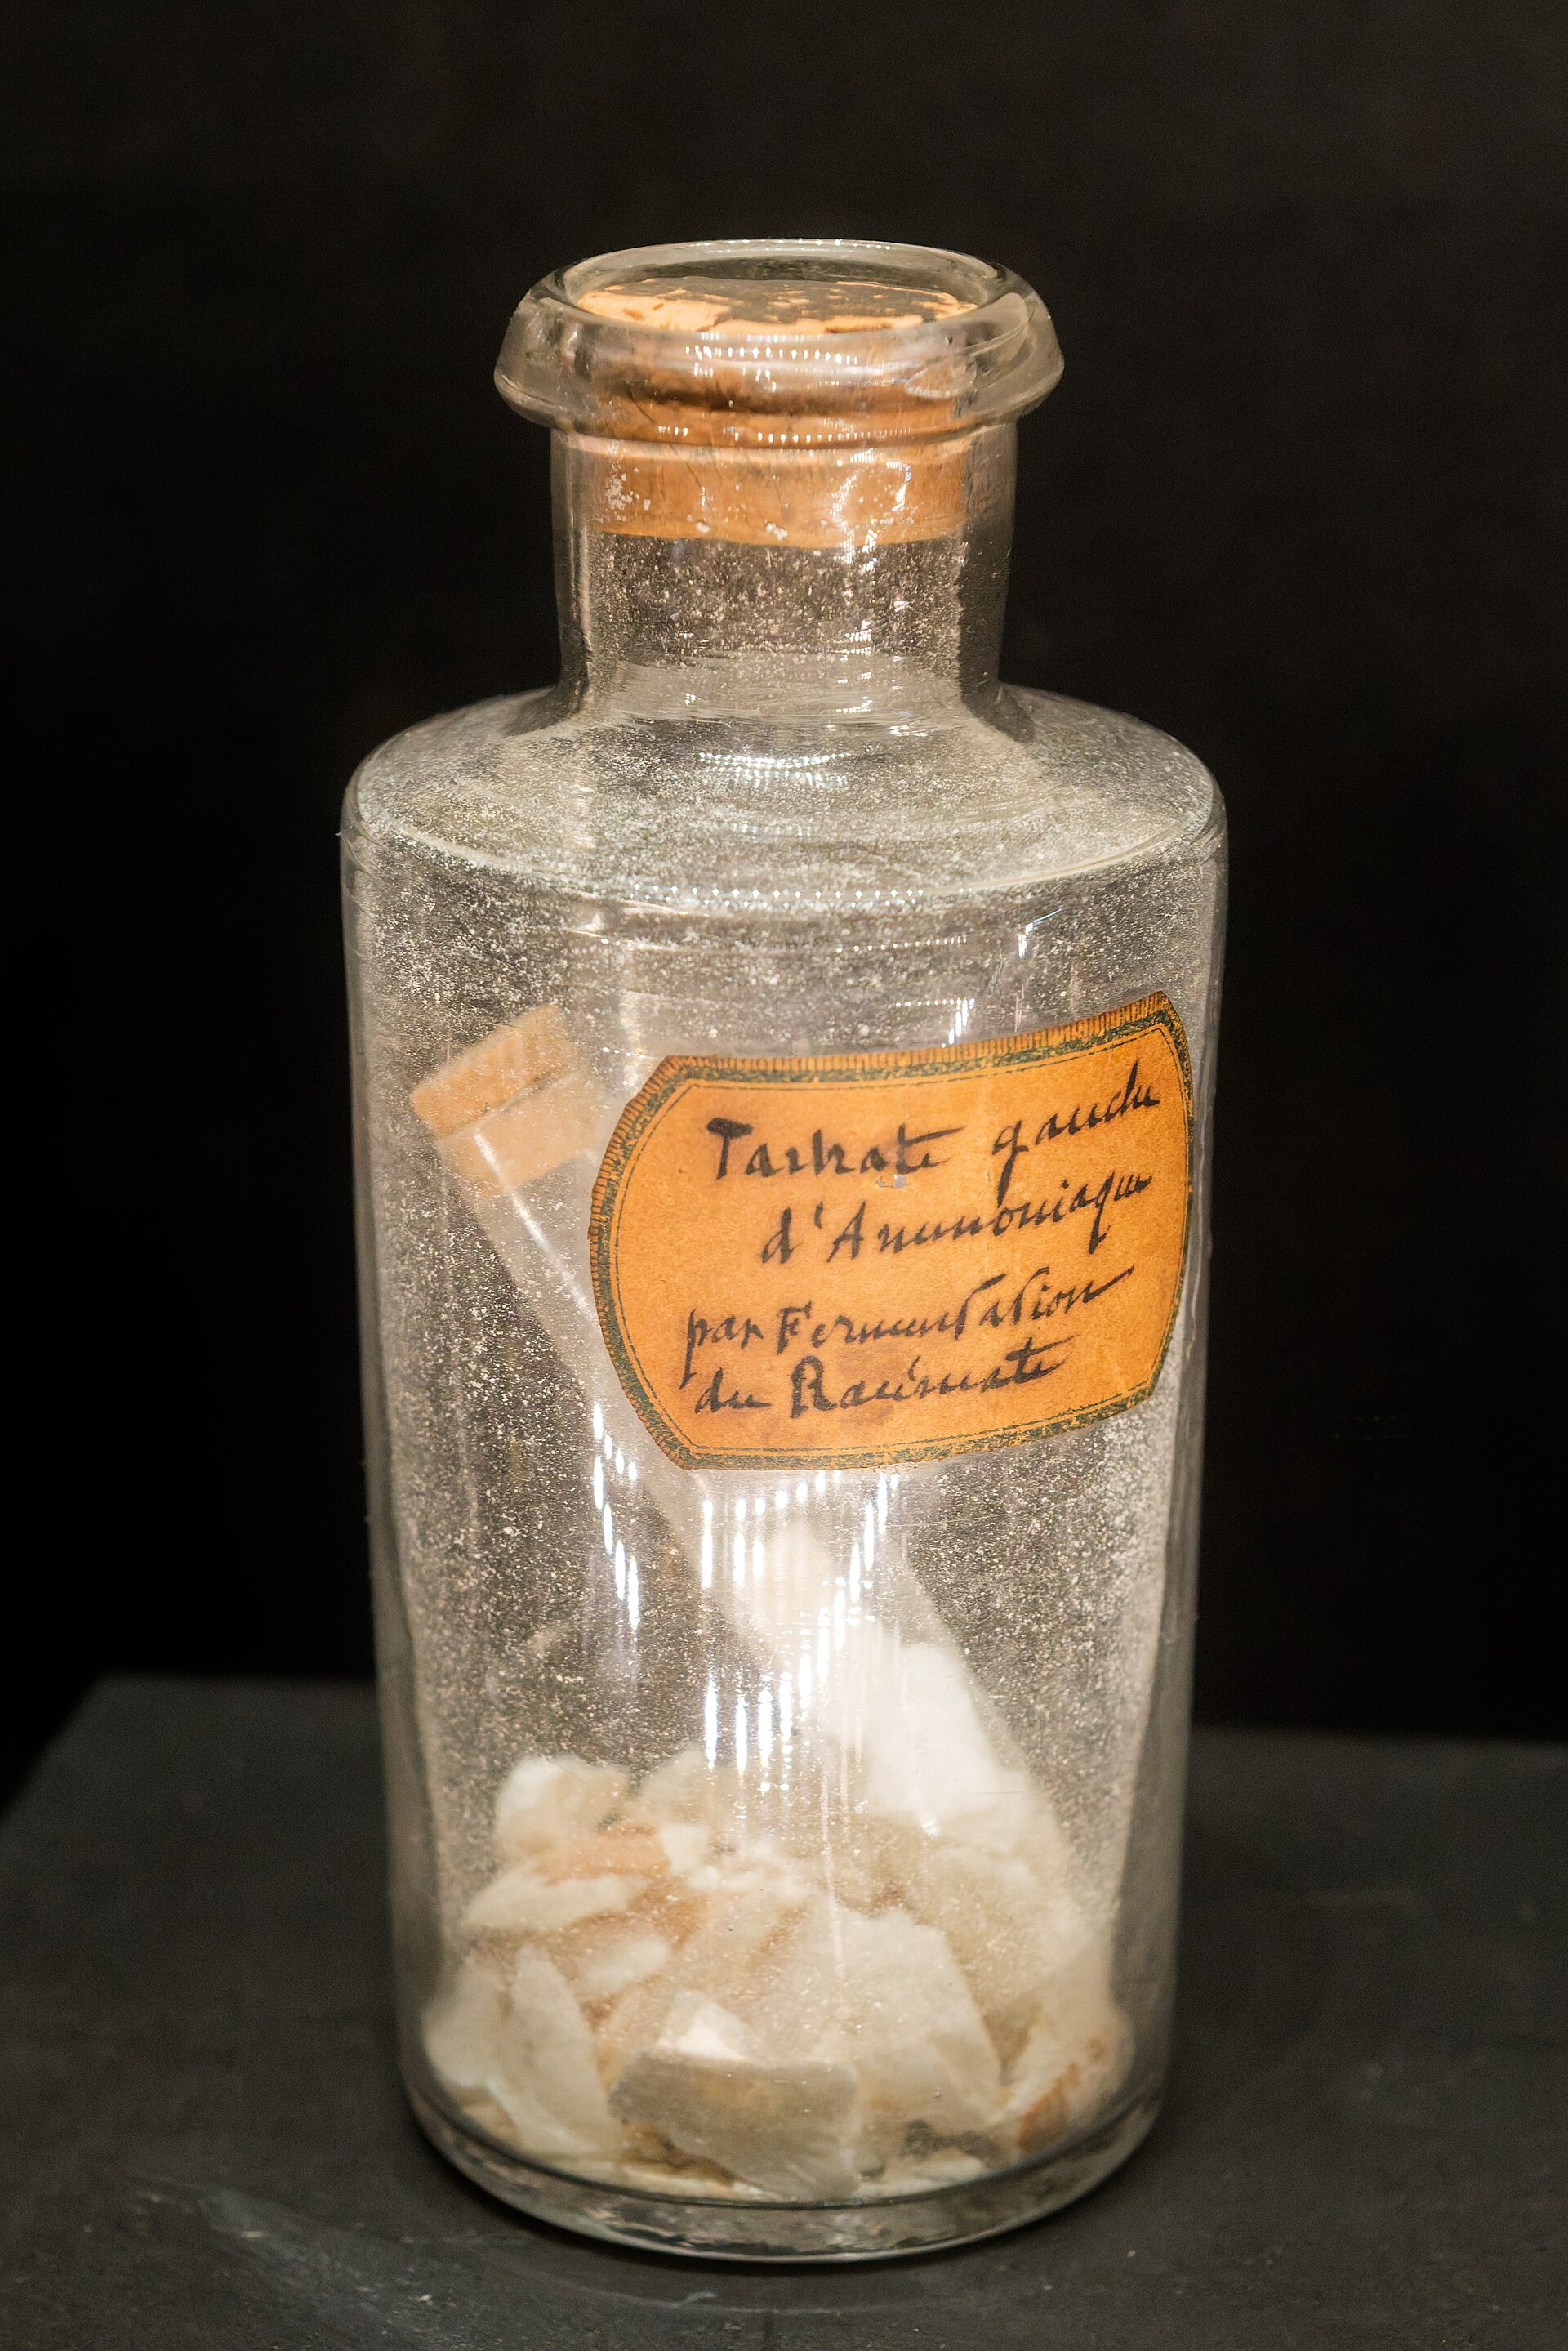
\includegraphics[height=5cm]{images/book1/tartrate-crystals.jpg}

{\small पाश्चर के संग्रह से अमोनियम टार्टरेट के क्रिस्टल। फ़ोटो:
मारी-लान ताय पामार, CC BY 4.0।}
\end{minipage}
\end{omfigure}

\section{Z और E समावयवी}


\begin{definition}[Z और E समावयवी]\label{def:g12:stereochemistry:z-e}
जब किसी \ce{C=C} \omterm{def:g10:lewis-and-shape:multiple-bond}{द्विआबंध} के हर कार्बन पर दो भिन्न \omterm{def:g7:atoms-and-molecules:atom}{परमाणु}
या समूह हों, तो दो \omterm{def:g12:stereochemistry:stereoisomer}{त्रिविम समावयवी} होते हैं, क्योंकि \omterm{def:g10:lewis-and-shape:multiple-bond}{द्विआबंध}
घूमता नहीं। हर कार्बन पर, वह समूह प्राथमिकता पाता है जिसके कार्बन से आबंधित \omterm{def:g7:atoms-and-molecules:atom}{परमाणु} का
\omterm{def:g9:inside-the-atom:atomic-number}{परमाणु क्रमांक} बड़ा हो। यदि प्राथमिकता वाले दोनों समूह \omterm{def:g10:lewis-and-shape:multiple-bond}{द्विआबंध} के एक ही
ओर हों, तो \omterm{def:g11:organic-skeletons:isomer}{समावयवी} \emph{Z}\index{Z समावयवी} है; यदि वे
विपरीत ओर हों, तो वह \emph{E}\index{E समावयवी} है।
\end{definition}

\begin{method}[Z या E?]\label{met:g12:stereochemistry:z-e}
\begin{enumerate}
  \item जाँचिए कि \omterm{def:g10:lewis-and-shape:multiple-bond}{द्विआबंध} के हर कार्बन पर दो भिन्न
        समूह हैं; अन्यथा कोई \omterm{def:g12:stereochemistry:z-e}{Z}/\omterm{def:g12:stereochemistry:z-e}{E} समावयवता नहीं है।
  \item हर कार्बन पर उस समूह को प्राथमिकता दीजिए जिसके पहले \omterm{def:g7:atoms-and-molecules:atom}{परमाणु} का
        \omterm{def:g9:inside-the-atom:atomic-number}{परमाणु क्रमांक} बड़ा हो (बराबरी की स्थिति के पूरे नियम
        विश्वविद्यालय के प्रथम वर्ष के खंड में दिए गए हैं)।
  \item एक ही ओर: \omterm{def:g12:stereochemistry:z-e}{Z}। विपरीत ओर: \omterm{def:g12:stereochemistry:z-e}{E}।
\end{enumerate}
\end{method}

\begin{omfigure}
\setchemfig{atom sep=2em}
\begin{tabular}{cc}
\chemfig{C(-[:150]H_3C)(-[:210]H)=C(-[:30]CH_3)(-[:-30]H)} &
\chemfig{C(-[:150]H_3C)(-[:210]H)=C(-[:30]H)(-[:-30]CH_3)} \\[4pt]
\small (\omterm{def:g12:stereochemistry:z-e}{Z})-ब्यूट-2-ईन: \ce{CH3} समूह एक ही ओर &
\small (\omterm{def:g12:stereochemistry:z-e}{E})-ब्यूट-2-ईन: \ce{CH3} समूह विपरीत ओर
\end{tabular}

{\small ब्यूट-2-ईन के दो \omterm{def:g12:stereochemistry:stereoisomer}{त्रिविम समावयवी}। हर कार्बन पर \ce{CH3}
(कार्बन, $Z = 6$) को \ce{H} ($Z = 1$) पर प्राथमिकता है। वे
\omterm{def:g12:stereochemistry:diastereomer}{अप्रतिबिंबरूपी} हैं: वे भिन्न तापों पर उबलते हैं।}
\end{omfigure}

\section{संरूपण}

\begin{definition}[संरूपण]\label{def:g12:stereochemistry:conformation}
किसी \omterm{def:g7:atoms-and-molecules:molecule}{अणु} के \omterm{def:g7:atoms-and-molecules:atom}{परमाणु} एकल आबंध के चारों ओर घूम सकते हैं। ऐसे घूर्णनों से
पहुँची गई हर व्यवस्था \omterm{def:g7:atoms-and-molecules:molecule}{अणु} का एक \emph{संरूपण}\index{संरूपण}
है। एक \omterm{def:g7:atoms-and-molecules:molecule}{अणु} के संरूपण \omterm{def:g11:organic-skeletons:isomer}{समावयवी} नहीं हैं: कमरे के ताप पर वे
लगातार एक-दूसरे में बदलते रहते हैं।
\end{definition}

\begin{omfigure}
\begin{tikzpicture}[font=\small]
  \pic (s) at (0,0) {omnewman={90}{30}};
  \foreach \k in {1,2,3} { \node at (s-f\k) {H}; \node at (s-b\k) {H}; }
  \node[anchor=north, align=center] at (0,-1.7) {सांतरित: दोनों कार्बनों के\\ H परमाणु बारी-बारी से आते हैं};
  \pic (e) at (5,0) {omnewman={90}{112}};
  \foreach \k in {1,2,3} { \node at (e-f\k) {H}; \node[black!60] at (e-b\k) {H}; }
  \node[anchor=north, align=center] at (5,-1.7) {ग्रसित: वे आमने-सामने\\ होते हैं (थोड़ा हटाकर बनाए गए)};
\end{tikzpicture}

{\small एथेन, \ce{CH3-CH3}, के दो \omterm{def:g12:stereochemistry:conformation}{संरूपण}, \ce{C-C} आबंध की सीध में देखे गए।
सामने वाला कार्बन केंद्र है, पीछे वाला कार्बन वृत्त।
सांतरित \omterm{def:g12:stereochemistry:conformation}{संरूपण}, जिसमें \omterm{def:g7:atoms-and-molecules:atom}{परमाणु} एक-दूसरे से सबसे दूर होते हैं, सबसे
स्थायी है।}
\end{omfigure}

\begin{remark}[यह क्यों मायने रखता है]\label{rem:g12:stereochemistry:matters}
सजीव \omterm{def:g12:stereochemistry:chiral}{किरैल} \omterm{def:g7:atoms-and-molecules:molecule}{अणुओं} (प्रोटीन, शर्कराएँ) से बने होते हैं, और उनसे बने
ग्राही और एंज़ाइम \omterm{def:g12:stereochemistry:enantiomer}{प्रतिबिंबरूपियों} में भेद करते हैं: दो
\omterm{def:g12:stereochemistry:enantiomer}{प्रतिबिंबरूपियों} की गंध, स्वाद या औषधि के रूप में क्रिया बहुत भिन्न हो सकती है। इसीलिए
\omterm{def:g12:stereochemistry:chiral}{असममित कार्बन} वाली दवा बनाने वाले रसायनज्ञों को पता होना चाहिए
कि वे कौन-सा \omterm{def:g12:stereochemistry:enantiomer}{प्रतिबिंबरूपी} बनाते हैं, और हर एक का परीक्षण करना चाहिए।
\end{remark}

\section{अभ्यास}

\begin{exercise}[$\star$]\label{exo:g12:stereochemistry:1}
इनमें से किन \omterm{def:g7:atoms-and-molecules:molecule}{अणुओं} में \omterm{def:g12:stereochemistry:chiral}{असममित कार्बन} है? उसे तारे से चिह्नित कीजिए।
ब्यूटेन-2-ऑल \ce{CH3-CH(OH)-CH2-CH3}; प्रोपेन-2-ऑल \ce{CH3-CH(OH)-CH3};
2-क्लोरोब्यूटेन; लैक्टिक अम्ल \ce{CH3-CH(OH)-COOH}।
\end{exercise}

\begin{exercise}[$\star$]\label{exo:g12:stereochemistry:2}
हर \omterm{def:g11:organic-skeletons:isomer}{समावयवी} \omterm{def:g12:stereochemistry:z-e}{Z} है या \omterm{def:g12:stereochemistry:z-e}{E}?
\begin{center}
\setchemfig{atom sep=1.8em}
\chemfig{C(-[:150]Cl)(-[:210]H)=C(-[:30]Cl)(-[:-30]H)} \qquad
\chemfig{C(-[:150]H_3C)(-[:210]H)=C(-[:30]H)(-[:-30]CH_2-CH_3)}
\end{center}
\end{exercise}

\begin{exercise}[$\star$]\label{exo:g12:stereochemistry:3}
इनमें से कौन \omterm{def:g12:stereochemistry:chiral}{किरैल} हैं: एक दस्ताना, एक चम्मच, एक पेंच, एक घन? \omterm{def:g7:atoms-and-molecules:molecule}{अणुओं}
\ce{CH2Cl2} और \ce{CHFClBr} में से कौन \omterm{def:g12:stereochemistry:chiral}{किरैल} है?
\end{exercise}

\begin{exercise}[$\star$]\label{exo:g12:stereochemistry:4}
\omterm{def:g12:stereochemistry:enantiomer}{रेसेमिक मिश्रण} क्या है? कार्वोन के मामले में, उससे पुदीने की गंध आती है, विलायती जीरे की,
या दोनों की?
\end{exercise}

\begin{exercise}[$\star$]\label{exo:g12:stereochemistry:5}
क्या ब्यूट-1-ईन \ce{CH2=CH-CH2-CH3} \omterm{def:g12:stereochemistry:z-e}{Z} और \omterm{def:g12:stereochemistry:z-e}{E समावयवियों} के रूप में हो सकती है? क्यों?
\end{exercise}

\begin{exercise}[$\star\star$]\label{exo:g12:stereochemistry:6}
\omterm{def:g12:stereochemistry:cram}{क्रैम निरूपण} में ब्यूटेन-2-ऑल के दोनों \omterm{def:g12:stereochemistry:enantiomer}{प्रतिबिंबरूपी} बनाइए, उनके
बीच एक दर्पण के साथ।
\end{exercise}

\begin{exercise}[$\star\star$]\label{exo:g12:stereochemistry:7}
इनके कितने \omterm{def:g12:stereochemistry:stereoisomer}{त्रिविम समावयवी} हैं: 2-क्लोरोब्यूटेन;
2,3-डाइक्लोरोब्यूटेन \ce{CH3-CHCl-CHCl-CH3}; पेंट-2-ईन
\ce{CH3-CH=CH-CH2-CH3}?
\end{exercise}

\begin{exercise}[$\star\star$]\label{exo:g12:stereochemistry:8}
बताइए कि ये जोड़े \omterm{def:g12:stereochemistry:enantiomer}{प्रतिबिंबरूपी} हैं, \omterm{def:g12:stereochemistry:diastereomer}{अप्रतिबिंबरूपी} हैं या एक ही
\omterm{def:g7:atoms-and-molecules:molecule}{अणु}: L- और D-टार्टरिक अम्ल; L- और मेसो-टार्टरिक अम्ल; (\omterm{def:g12:stereochemistry:z-e}{Z})- और
(\omterm{def:g12:stereochemistry:z-e}{E})-ब्यूट-2-ईन; मेसो-टार्टरिक अम्ल और उसका अपना दर्पण-प्रतिबिंब।
\end{exercise}

\begin{exercise}[$\star\star$]\label{exo:g12:stereochemistry:9}
ब्यूटेन, \ce{CH3-CH2-CH2-CH3}, को उसके केंद्रीय आबंध की सीध में देखा जाता है। वह
सांतरित \omterm{def:g12:stereochemistry:conformation}{संरूपण} बनाइए जिसमें दोनों \ce{CH3} समूह विपरीत हों, और
एक ग्रसित \omterm{def:g12:stereochemistry:conformation}{संरूपण} जिसमें वे आमने-सामने हों। कौन-सा अधिक स्थायी है?
क्यों?
\end{exercise}

\begin{exercise}[$\star\star$]\label{exo:g12:stereochemistry:10}
मेसो-टार्टरिक अम्ल में दो \omterm{def:g12:stereochemistry:chiral}{असममित कार्बन} हैं पर वह \omterm{def:g12:stereochemistry:chiral}{किरैल} नहीं है।
उसके दर्पण-तल की मदद से समझाइए।
\end{exercise}

\begin{exercise}[$\star\star$]\label{exo:g12:stereochemistry:11}
पेंट-2-ईन के \omterm{def:g12:stereochemistry:z-e}{Z} और \omterm{def:g12:stereochemistry:z-e}{E समावयवी} बनाइए और उनके नाम लिखिए।
\end{exercise}

\begin{exercise}[$\star\star\star$]\label{exo:g12:stereochemistry:12}
2,3-डाइब्रोमोब्यूटेन \ce{CH3-CHBr-CHBr-CH3} में दो \omterm{def:g12:stereochemistry:chiral}{असममित कार्बन} हैं।
टार्टरिक अम्ल के लिए इस्तेमाल किए गए टेढ़े-मेढ़े निरूपण में उसके \omterm{def:g12:stereochemistry:stereoisomer}{त्रिविम समावयवी}
बनाइए, और दिखाइए कि उनमें से एक मेसो रूप है।
\end{exercise}

\begin{exercise}[$\star\star\star$]\label{exo:g12:stereochemistry:13}
एक दवा के \omterm{def:g7:atoms-and-molecules:molecule}{अणु} में एक \omterm{def:g12:stereochemistry:chiral}{असममित कार्बन} है। उसका \omterm{def:g10:synthesis-yield:synthesis}{संश्लेषण} एक \omterm{def:g12:stereochemistry:enantiomer}{रेसेमिक
मिश्रण} देता है, पर केवल एक \omterm{def:g12:stereochemistry:enantiomer}{प्रतिबिंबरूपी} उस \omterm{def:g12:stereochemistry:chiral}{किरैल} ग्राही में फ़िट होता है जिस पर उसे
क्रिया करनी है। रेसेमिक दवा का कितना भाग सक्रिय है? दो तरीके बताइए जिनसे
कोई रसायनज्ञ बेहतर कर सकता है।
\end{exercise}

\begin{exercise}[$\star\star\star$]\label{exo:g12:stereochemistry:14}
हेक्सा-2,4-डाइईन, \ce{CH3-CH=CH-CH=CH-CH3}, में दो \omterm{def:g10:lewis-and-shape:multiple-bond}{द्विआबंध} हैं, जिनमें से हर एक
\omterm{def:g12:stereochemistry:z-e}{Z} या \omterm{def:g12:stereochemistry:z-e}{E} हो सकता है। इसके कितने \omterm{def:g12:stereochemistry:stereoisomer}{त्रिविम समावयवी} हैं? (\omterm{def:g7:atoms-and-molecules:molecule}{अणु} की
सममिति से सावधान रहिए।)
\end{exercise}

\begin{exercise}[$\star\star\star$]\label{exo:g12:stereochemistry:15}
एक शर्करा \omterm{def:g7:atoms-and-molecules:molecule}{अणु} में तीन \omterm{def:g12:stereochemistry:chiral}{असममित कार्बन} हैं और कोई सममिति नहीं। उसके अधिक से अधिक कितने
\omterm{def:g12:stereochemistry:stereoisomer}{त्रिविम समावयवी} हो सकते हैं? यह \omterm{def:g12:stereochemistry:enantiomer}{प्रतिबिंबरूपियों} के कितने जोड़े हैं?
हर \omterm{def:g12:stereochemistry:stereoisomer}{त्रिविम समावयवी} के कितने \omterm{def:g12:stereochemistry:diastereomer}{अप्रतिबिंबरूपी} हैं?
\end{exercise}

\section{समस्या: पाश्चर के क्रिस्टल}


\begin{problem}[{सप्ताहांत समस्या --- टार्टरिक अम्ल में दो असममित
कार्बन हैं: उसके वास्तव में कितने त्रिविम समावयवी हैं?}]
\label{pb:g12:stereochemistry:1}
% ledger: mp:tartaric-L, aw:C, aw:H, aw:O
टार्टरिक अम्ल, \ce{HOOC-CH(OH)-CH(OH)-COOH}, के रूपों ने इस खोज में
निर्णायक भूमिका निभाई कि \omterm{def:g7:atoms-and-molecules:molecule}{अणुओं} में हस्तता हो सकती है। L-टार्टरिक अम्ल लगभग \qty{169}{\celsius} पर पिघलता है।

\medskip
\noindent\textbf{भाग I --- \omterm{def:g7:atoms-and-molecules:molecule}{अणु}।}
\begin{enumerate}
  \item टार्टरिक अम्ल का \omterm{def:g11:organic-skeletons:formulas}{आण्विक सूत्र} और उसका \omterm{def:g10:the-mole:molar-mass}{मोलर द्रव्यमान} बताइए।
  \item उसके \omterm{def:g11:functional-groups:functional-group}{क्रियात्मक समूहों} के नाम बताइए, और हर एक कितने हैं।
  \item कौन-से कार्बन \omterm{def:g7:atoms-and-molecules:atom}{परमाणु} असममित हैं? हर एक के चार समूहों की सूची बनाइए।
  \item इस अध्याय के नियम के अनुसार, उसके अधिक से अधिक कितने \omterm{def:g12:stereochemistry:stereoisomer}{त्रिविम समावयवी}
        हो सकते हैं?
\end{enumerate}

\medskip
\noindent\textbf{भाग II --- \omterm{def:g12:stereochemistry:stereoisomer}{त्रिविम समावयवी}।}
\begin{enumerate}[resume]
  \item L-टार्टरिक अम्ल के टेढ़े-मेढ़े चित्र में \ce{OH} समूह
        ठोस पच्चरों से बनाए गए हैं या डैश वाले पच्चरों से?
  \item उसका दर्पण-प्रतिबिंब बनाइए। क्या दोनों अध्यारोपित हो सकते हैं? दर्पण-प्रतिबिंब
        का नाम बताइए।
  \item एक ठोस और एक डैश वाले पच्चर वाला रूप बनाइए। उसे मन ही मन केंद्रीय आबंध
        के चारों ओर घुमाइए, और एक दर्पण-तल खोजिए।
  \item क्या यह रूप \omterm{def:g12:stereochemistry:chiral}{किरैल} है? इसे क्या कहते हैं?
  \item समझाइए कि टार्टरिक अम्ल के केवल तीन \omterm{def:g12:stereochemistry:stereoisomer}{त्रिविम समावयवी} क्यों हैं।
  \item बताइए कि L और D, फिर L और मेसो, \omterm{def:g12:stereochemistry:enantiomer}{प्रतिबिंबरूपी} हैं या
        \omterm{def:g12:stereochemistry:diastereomer}{अप्रतिबिंबरूपी}।
\end{enumerate}

\medskip
\noindent\textbf{भाग III --- गुण।}
\begin{enumerate}[resume]
  \item D-टार्टरिक अम्ल किस ताप पर पिघलता है? क्यों?
  \item क्या मेसो-टार्टरिक अम्ल को उसी ताप पर पिघलना चाहिए? क्यों?
  \item कार्वोन दिखाता है कि दो \omterm{def:g12:stereochemistry:enantiomer}{प्रतिबिंबरूपियों} की गंध भिन्न हो सकती है। नाक
        उन्हें अलग क्यों पहचान सकती है जबकि थर्मामीटर नहीं?
  \item L और D टार्टरिक अम्ल का \omterm{def:g12:stereochemistry:enantiomer}{रेसेमिक मिश्रण}: क्या वह \omterm{def:g6:pure-substances-and-mixtures:pure-substance}{शुद्ध
        पदार्थ} है? क्या वह समग्र रूप से ध्रुवण-घूर्णक है?
\end{enumerate}

\medskip
\noindent\textbf{भाग IV --- पाश्चर।}
\begin{enumerate}[resume]
  \item पाश्चर के रेसेमिक लवण ने दो दर्पण-प्रतिबिंब आकृतियों के क्रिस्टल दिए।
        हर क्रिस्टल में क्या था?
  \item रेसेमिक लवण के \qty{10.0}{g} से वे हर प्रकार के
        क्रिस्टल के कितने द्रव्यमान की अपेक्षा कर सकते थे?
  \item इन क्रिस्टलों में मेसो रूप कभी क्यों नहीं दिखता?
  \item छाँटने के बाद वे कैसे जाँच सकते थे कि दोनों ढेर
        \omterm{def:g12:stereochemistry:enantiomer}{प्रतिबिंबरूपी} थे?
  \item 3-क्लोरोब्यूटेन-2-ऑल, \ce{CH3-CHCl-CH(OH)-CH3}, में भी दो
        \omterm{def:g12:stereochemistry:chiral}{असममित कार्बन} हैं। उसके कितने \omterm{def:g12:stereochemistry:stereoisomer}{त्रिविम समावयवी} हैं? वह
        टार्टरिक अम्ल की तरह एक क्यों नहीं खोता?
  \item अंतिम उत्तर बताइए: टार्टरिक अम्ल के कितने \omterm{def:g12:stereochemistry:stereoisomer}{त्रिविम समावयवी}
        हैं?
\end{enumerate}
\end{problem}
